\documentclass{article}
\usepackage{graphicx}
\usepackage{amsmath, amssymb}
\usepackage{booktabs}
\usepackage{hyperref}
\usepackage{caption}
\usepackage{geometry}
\geometry{margin=1in}

\title{Machine Learning Homework 3\\Dai Xunlian 225040015}
\author{225040015@link.cuhk.edu.cn}
\date{November 5, 2025}

\begin{document}
\maketitle

\section*{Overview}
This report documents solutions and results for three problems. All required figures are embedded directly from the generated PDF outputs in the \texttt{code release} directory. Final numerical results are summarized from the printed outputs recorded at the end of each Python file.

\section{Problem 1: Polynomial Regression and Ridge Regularization}
\subsection*{Setup}
We fit a polynomial model of degree 8 to the provided training data, and evaluate on the test set. Let \(X \in \mathbb{R}^{n\times 9}\) be the Vandermonde matrix up to degree 8, and \(y \in \mathbb{R}^n\) be the targets. The least squares estimator is \(\hat{\theta} = (X^\top X)^{-1}X^\top y\). For ridge with regularization parameter \(\lambda > 0\), we use \(\hat{\theta}_\lambda = (X^\top X + \lambda I)^{-1}X^\top y\).

\subsection*{Fitted Curve (Unregularized)}
\begin{figure}[h]
  \centering
  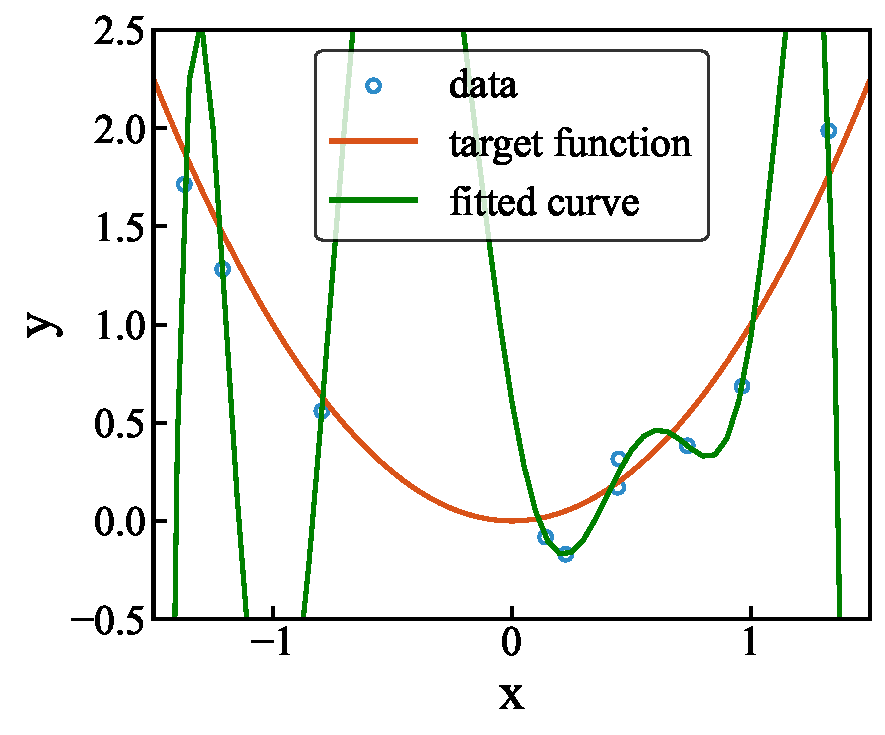
\includegraphics[width=0.8\linewidth]{code release/p1/a2_fitted_curve.pdf}
  \caption{Unregularized degree-8 fit with training data and target function.}
\end{figure}

\subsection*{Cross-Validation for \(\lambda\)}
\begin{figure}[h]
  \centering
  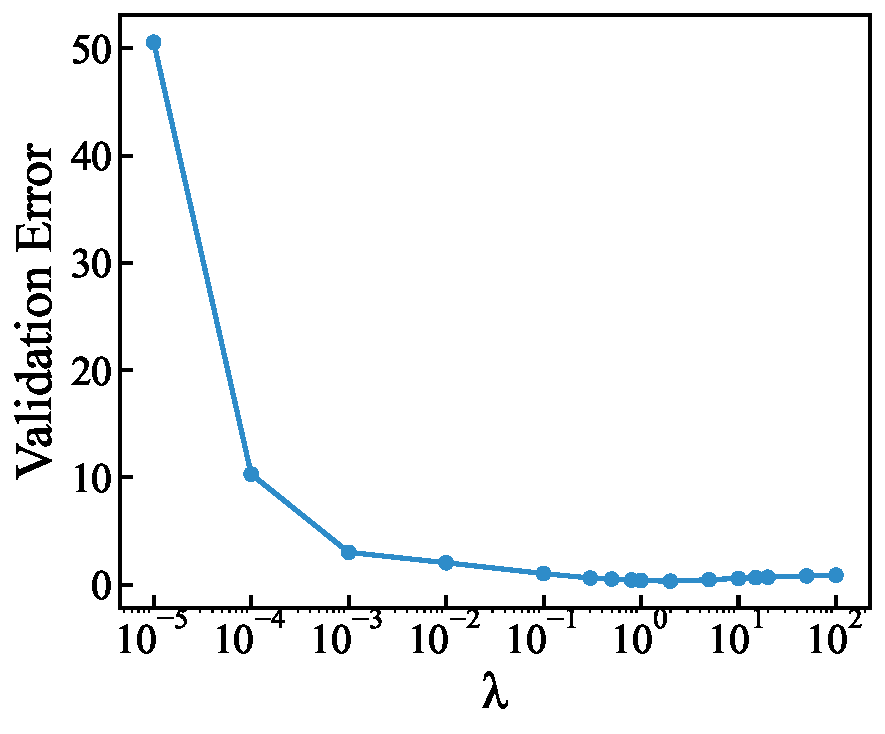
\includegraphics[width=0.7\linewidth]{code release/p1/b1_validation_error.pdf}
  \caption{Validation error vs. \(\lambda\) (log-scale).}
\end{figure}

\subsection*{Effect of \(\lambda\) on Fitted Curve}
\begin{figure}[h]
  \centering
  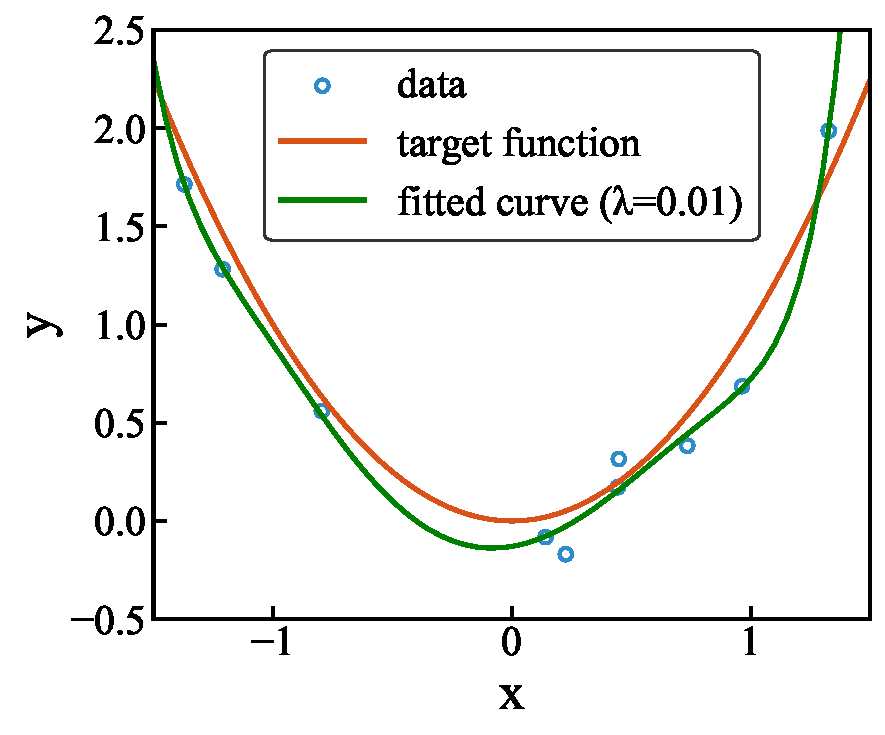
\includegraphics[width=0.45\linewidth]{code release/p1/b2_lambda_0.01.pdf}\hfill
  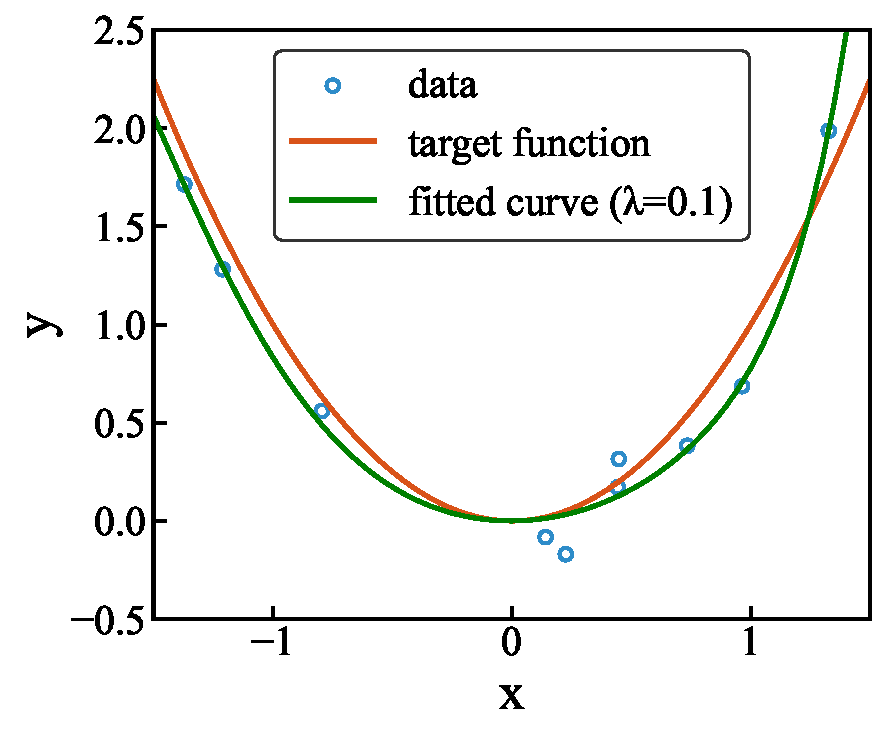
\includegraphics[width=0.45\linewidth]{code release/p1/b2_lambda_0.1.pdf}\\[0.8em]
  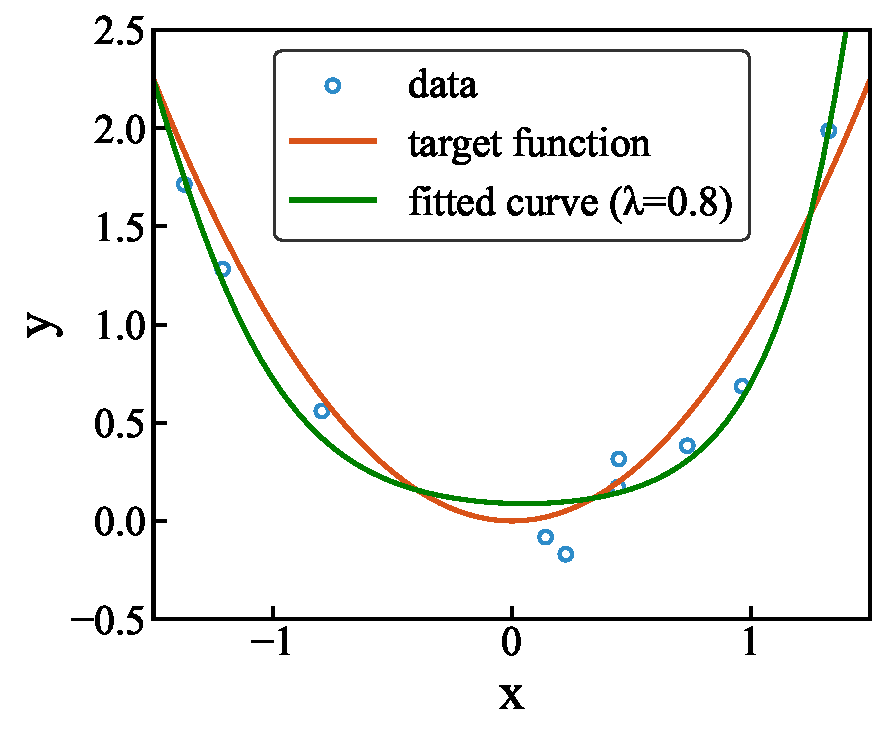
\includegraphics[width=0.45\linewidth]{code release/p1/b2_lambda_0.8.pdf}\hfill
  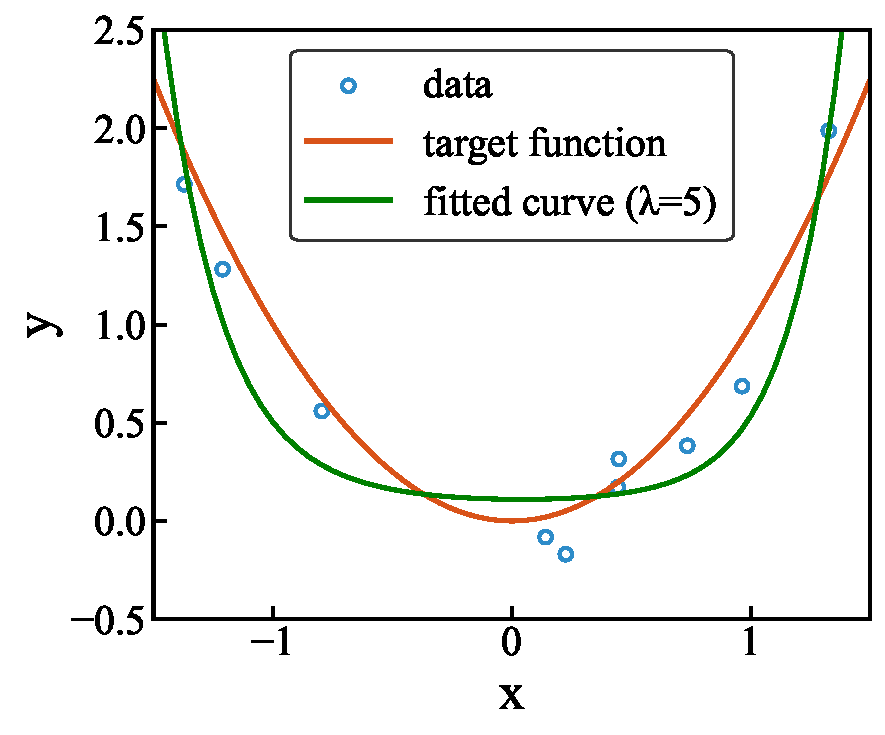
\includegraphics[width=0.45\linewidth]{code release/p1/b2_lambda_5.pdf}
  \caption{Fitted curves under different \(\lambda\) values.}
\end{figure}

\subsection*{Key Numerical Results}
From the program output:
\begin{itemize}
  \item Test error (unregularized, part a3): \textbf{4.5607}
  \item Ridge test error: \(\lambda=0.01\): \textbf{0.6634}\;\; \(\lambda=0.1\): \textbf{0.6341}\;\; \(\lambda=0.8\): \textbf{0.6493}\;\; \(\lambda=5\): \textbf{0.8207}
\end{itemize}

\section{Problem 2: PCA on ORL Faces}
\subsection*{Top Eigenfaces}
\begin{figure}[h]
  \centering
  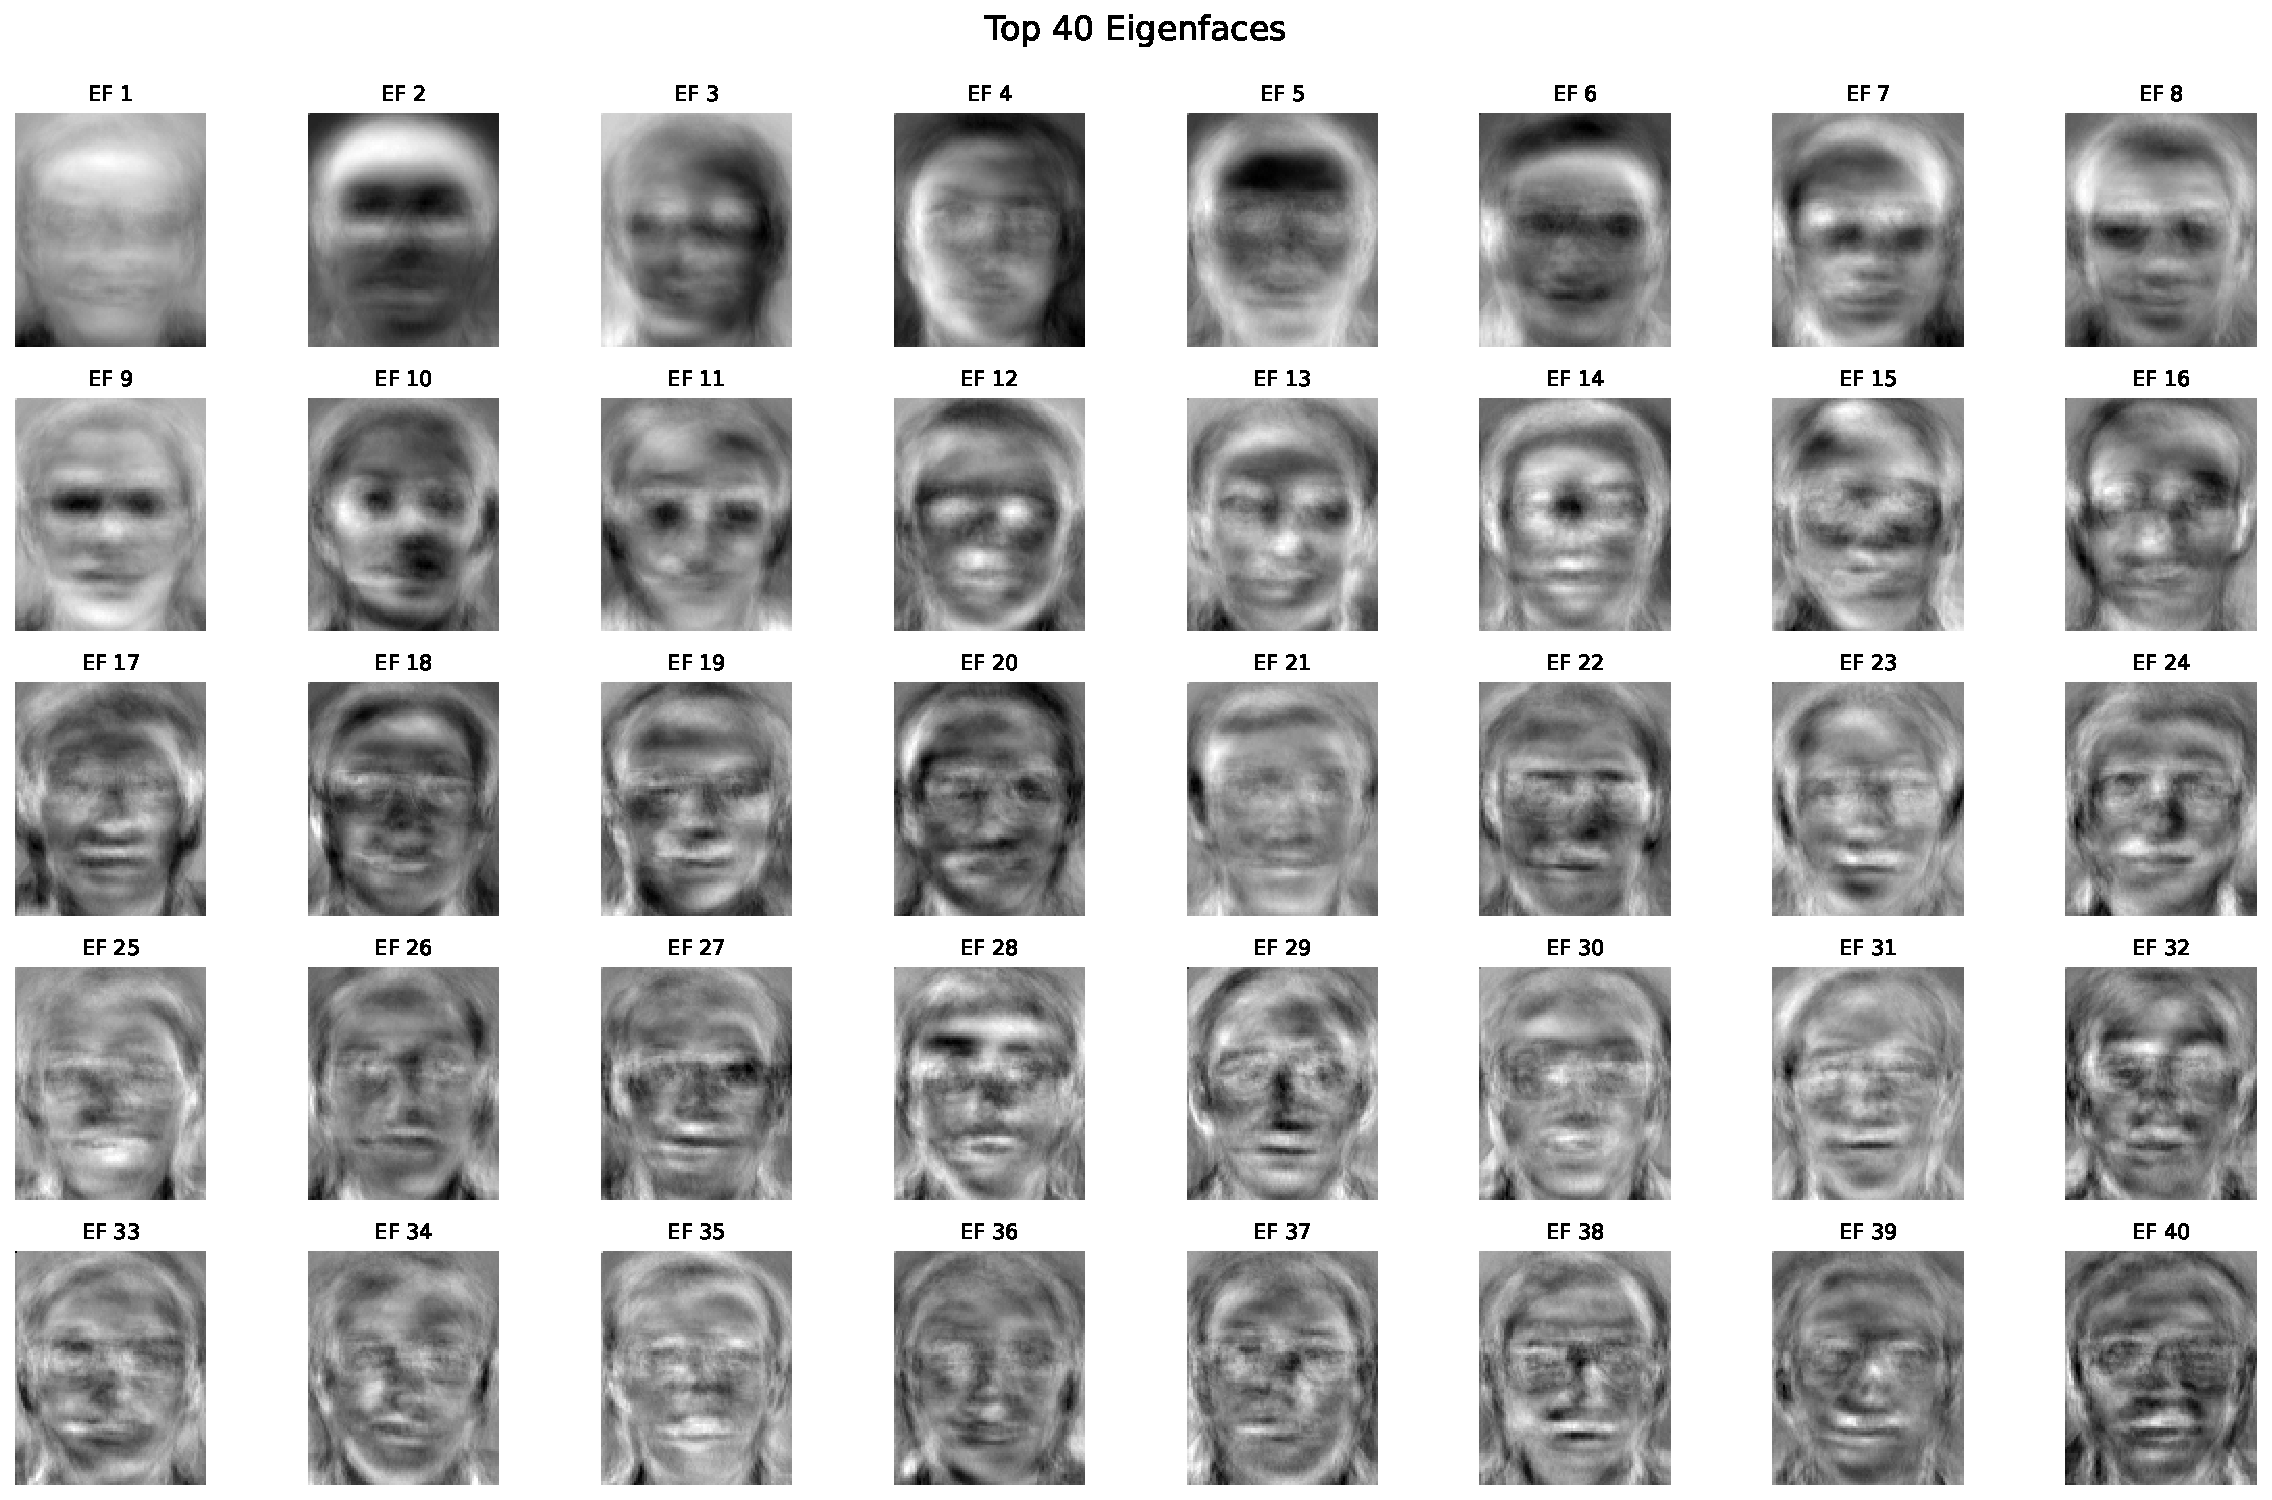
\includegraphics[width=0.95\linewidth]{code release/p2/eigenfaces_top40.pdf}
  \caption{Top 40 eigenfaces learned by PCA.}
\end{figure}

\subsection*{Reconstruction with Varying \(k\)}
\begin{figure}[h]
  \centering
  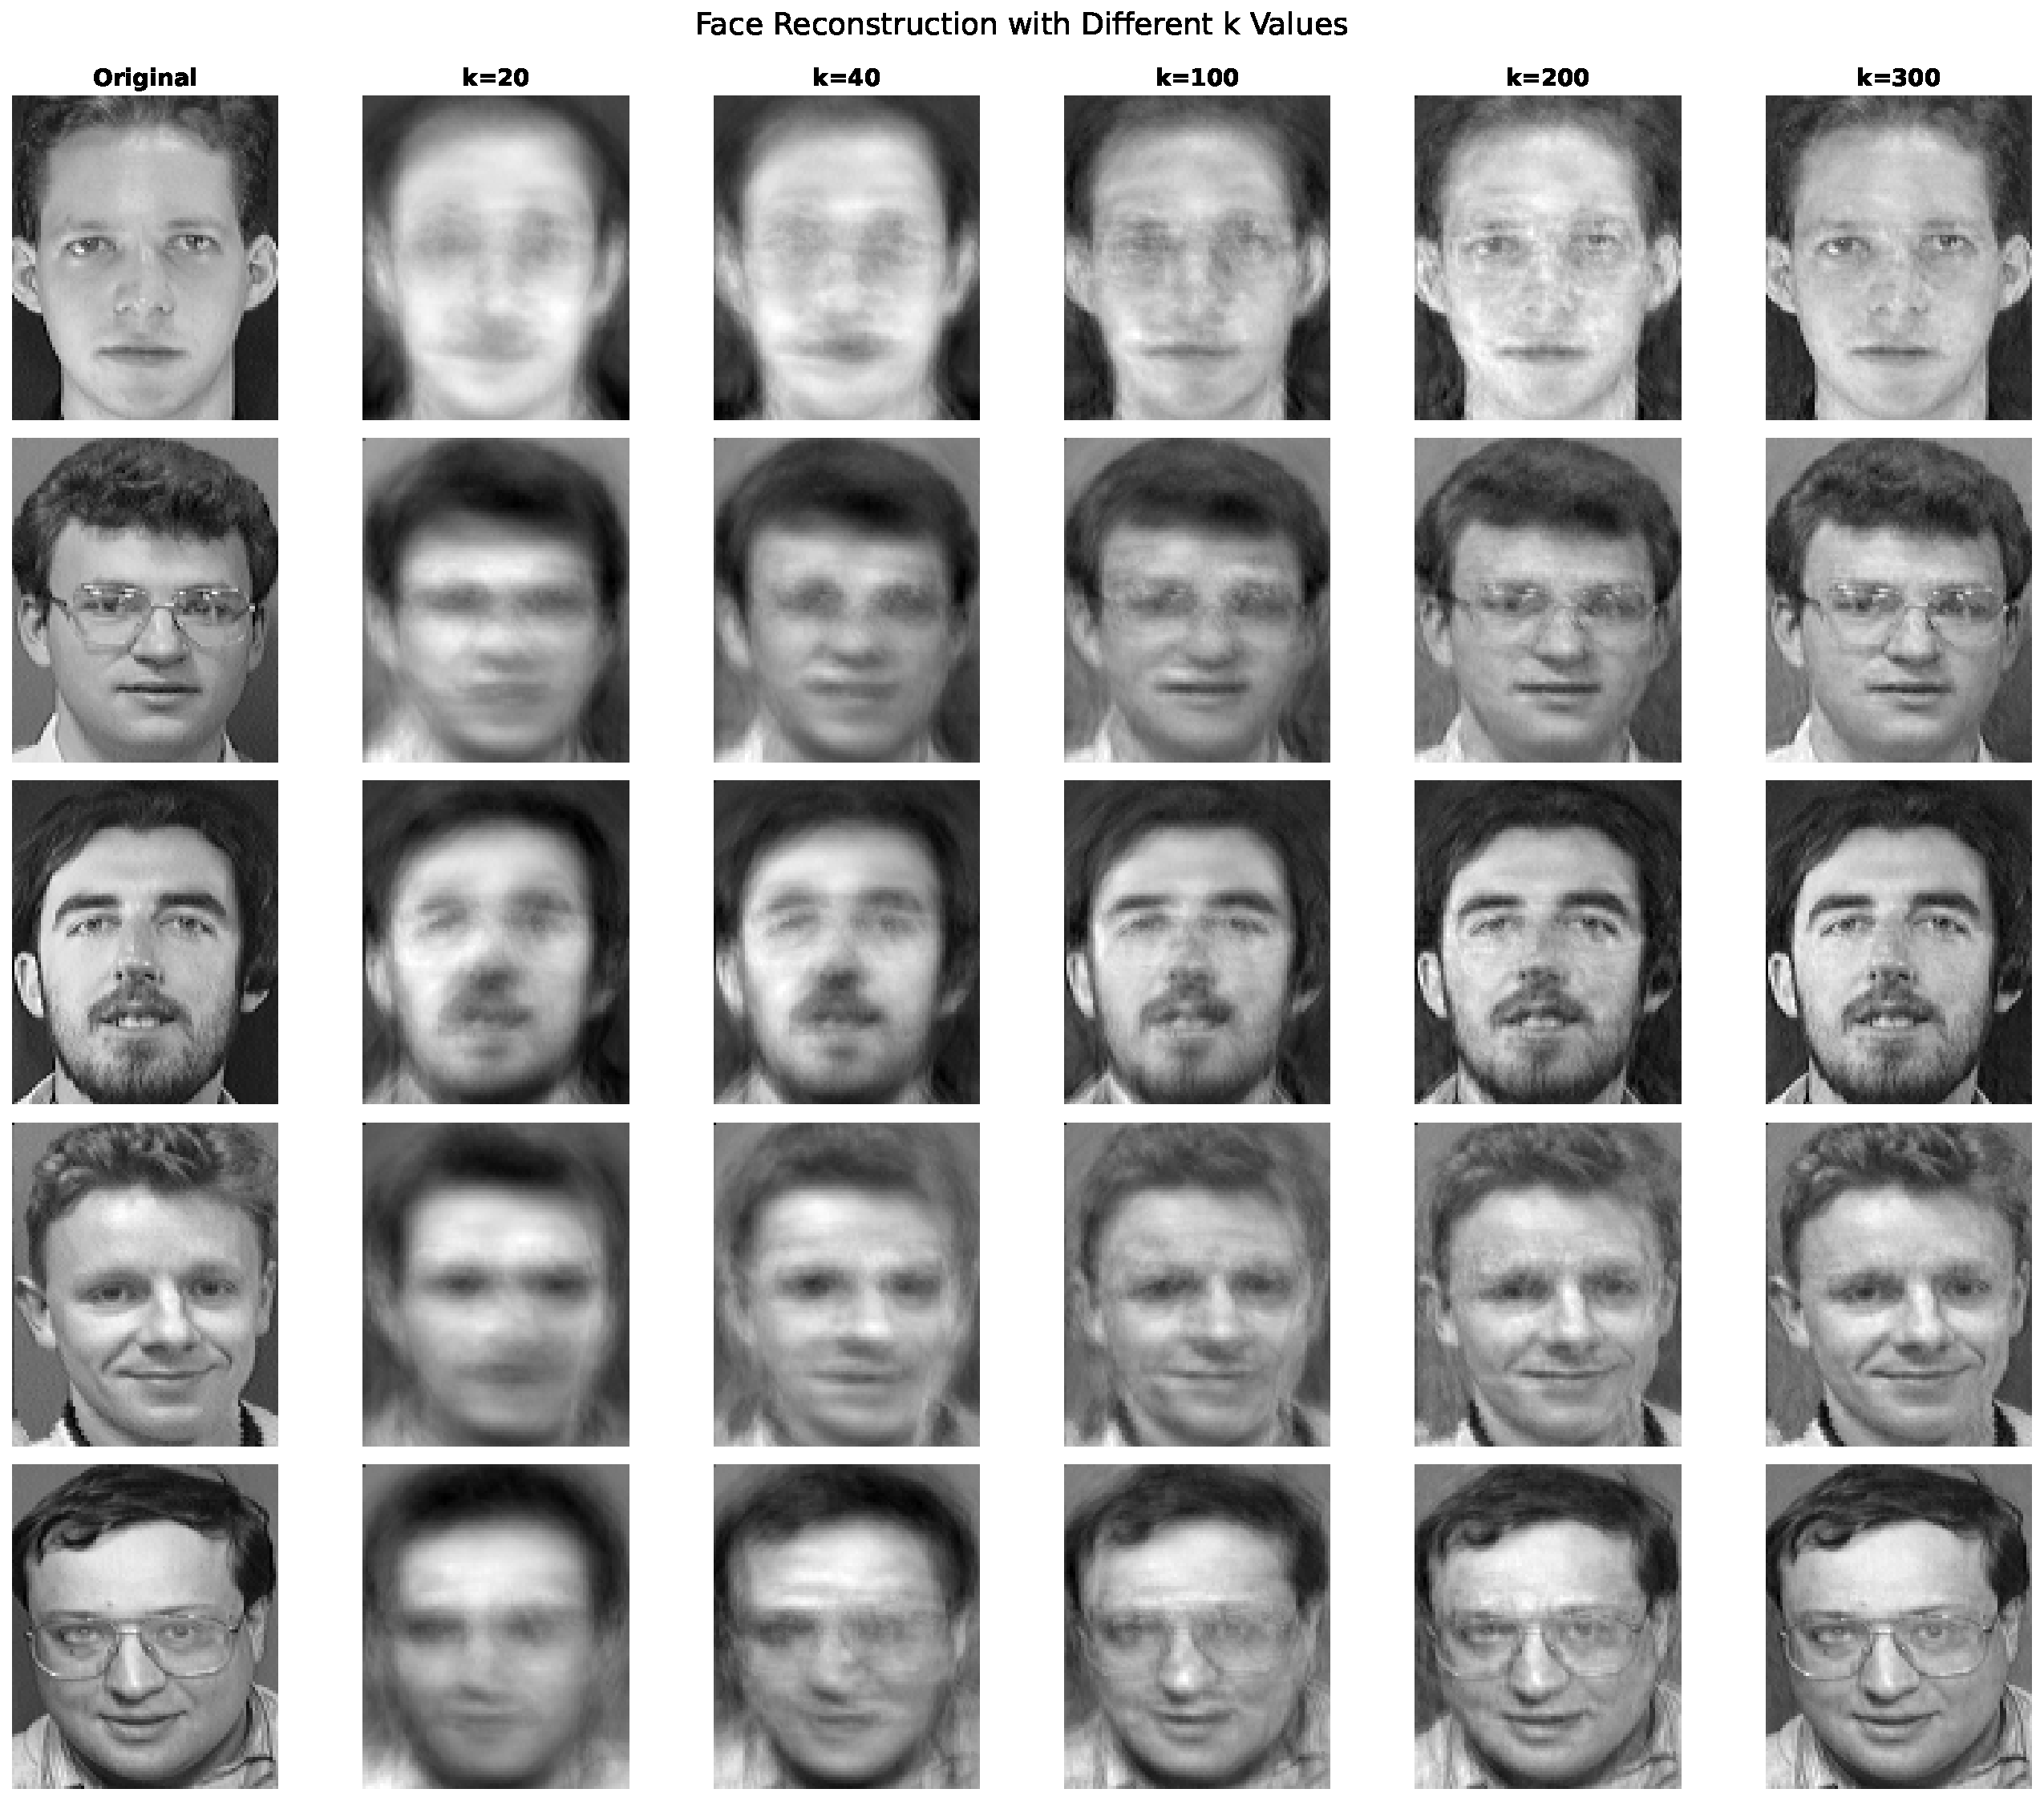
\includegraphics[width=0.95\linewidth]{code release/p2/reconstruction_comparison.pdf}
  \caption{Reconstruction of selected images with \(k \in \{20,40,100,200,300\}\).}
\end{figure}

\subsection*{SNR vs Number of Components}
\begin{figure}[h]
  \centering
  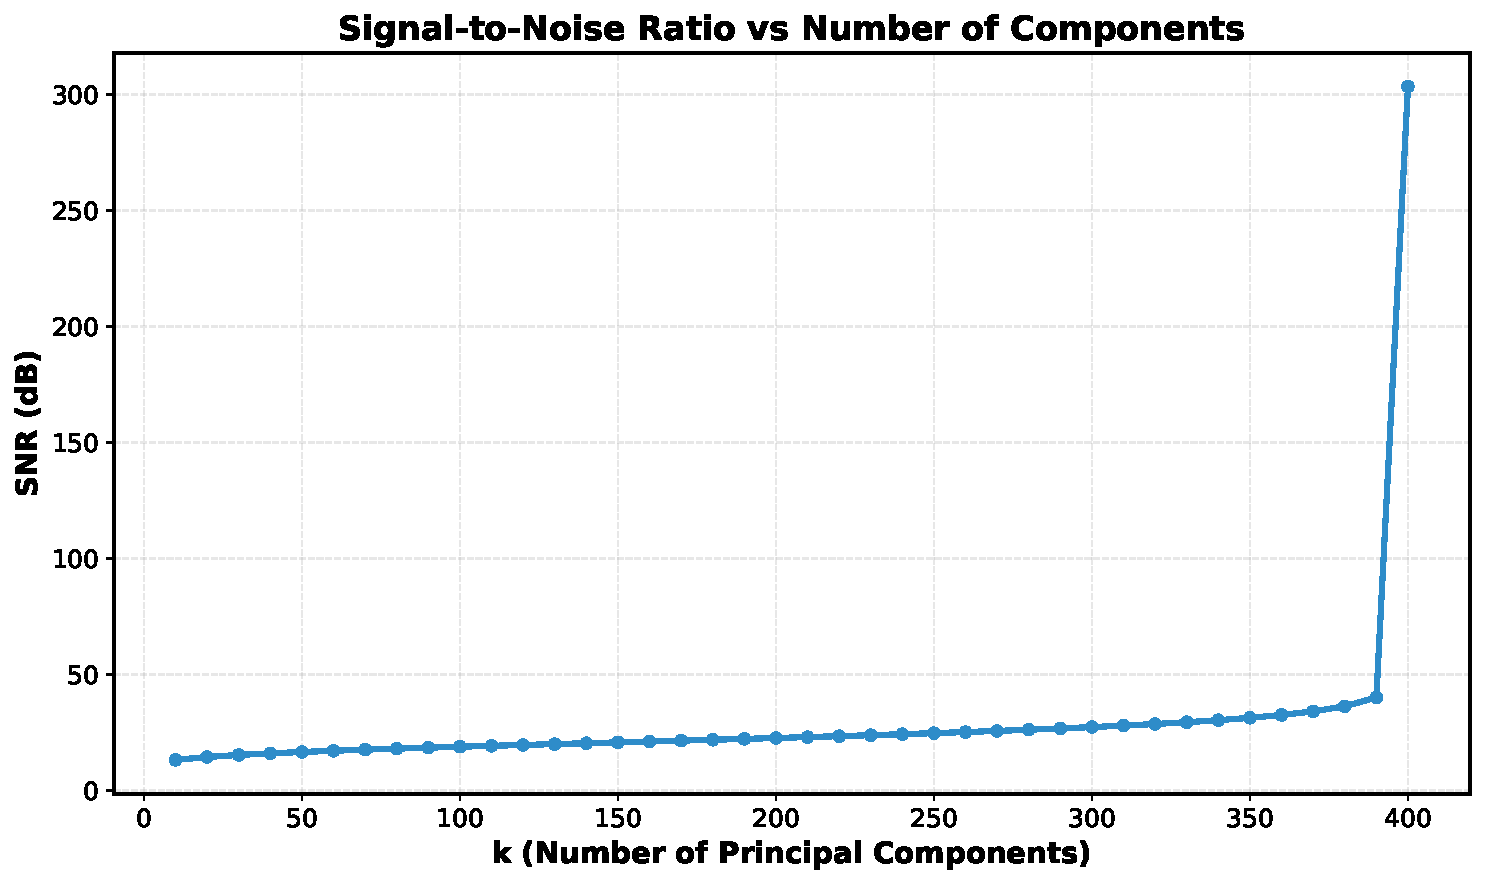
\includegraphics[width=0.85\linewidth]{code release/p2/snr_vs_k.pdf}
  \caption{SNR as a function of the number of principal components.}
\end{figure}

\subsection*{Key Numerical Results}
From the program output:
\begin{itemize}
  \item SNR samples: \(k=20\): \textbf{14.53 dB}, \(k=40\): \textbf{16.08 dB}, \(k=100\): \textbf{18.93 dB}, \(k=200\): \textbf{22.69 dB}, \(k=300\): \textbf{27.40 dB}
  \item Variance explained: Top 20: \textbf{70.60\%}, Top 40: \textbf{79.23\%}, Top 100: \textbf{89.10\%}, Top 200: \textbf{95.38\%}, Top 300: \textbf{98.43\%}
\end{itemize}
Intuitively, larger \(k\) retains more variance, improving reconstruction fidelity and SNR.

\section{Problem 3: SVM on MNIST}
\subsection*{Part (a): Polynomial Kernels}
We train SVMs with polynomial kernels of degrees 1 and 2. The validation error as a function of \(C\) is shown below.

\begin{figure}[h]
  \centering
  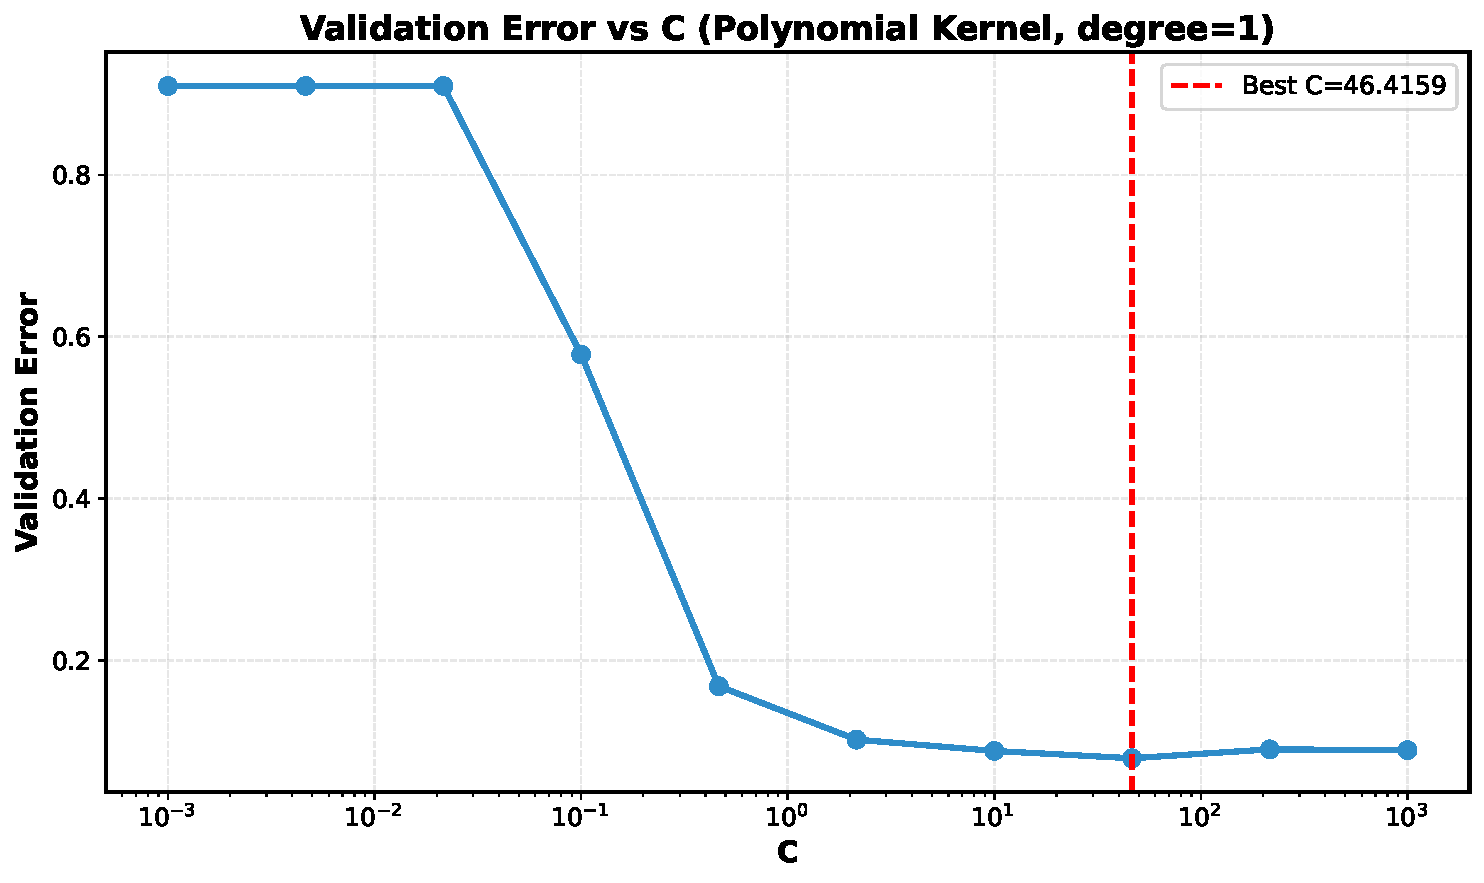
\includegraphics[width=0.8\linewidth]{code release/p3/poly_degree1_validation_error.pdf}
  \caption{Validation error vs. \(C\) for polynomial kernel (degree 1).}
\end{figure}

\begin{figure}[h]
  \centering
  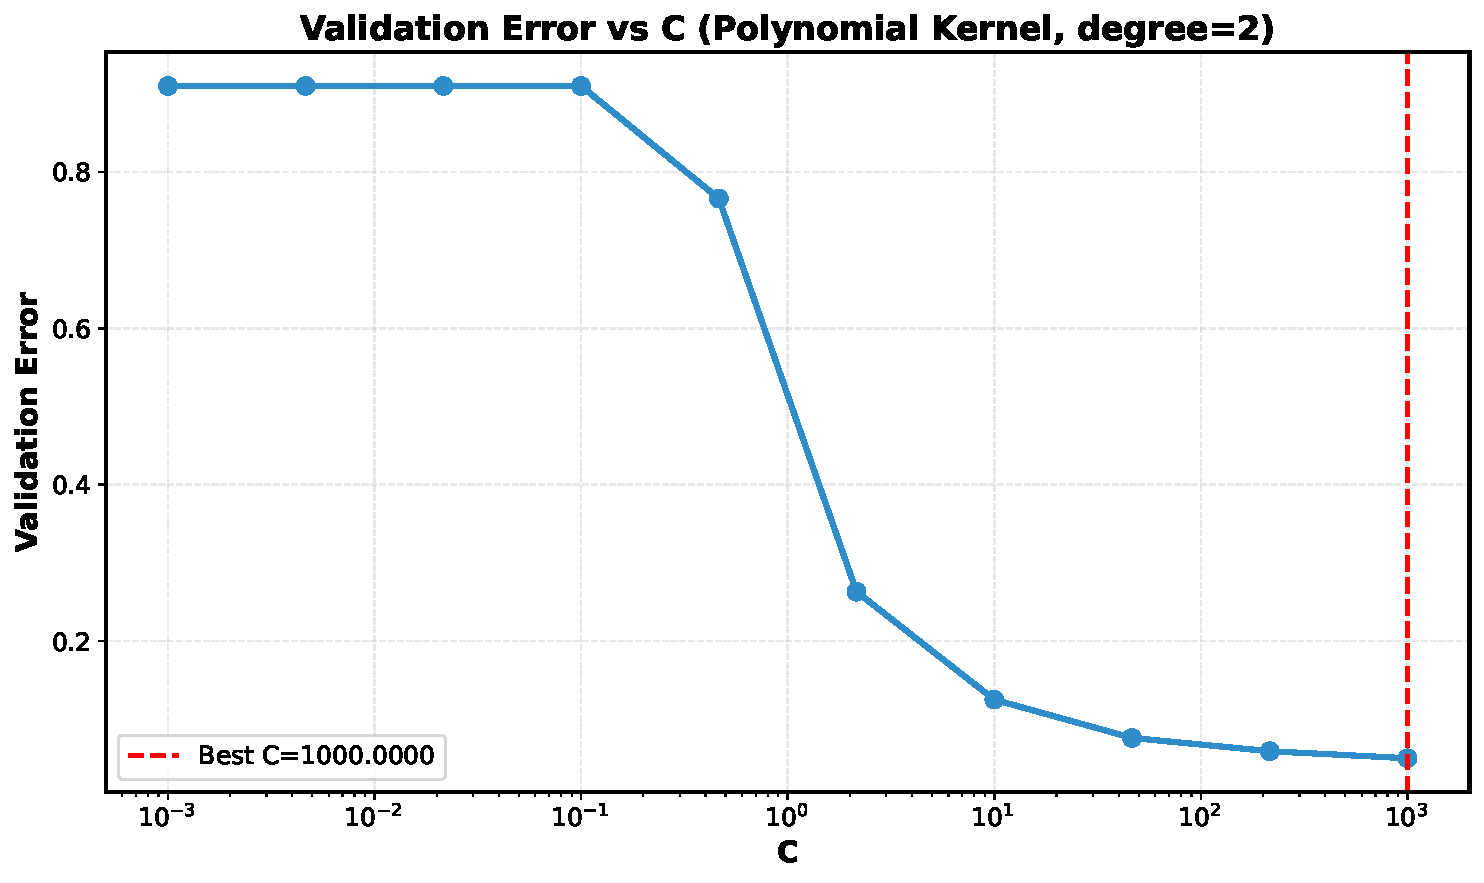
\includegraphics[width=0.8\linewidth]{code release/p3/poly_degree2_validation_error.pdf}
  \caption{Validation error vs. \(C\) for polynomial kernel (degree 2).}
\end{figure}

Key results from the output:
\begin{itemize}
  \item Degree 1: Best \(C=46.4159\), Best Val Error: \textbf{0.0790}, Test Error: \textbf{0.1097}, Test Acc: \textbf{0.8903}
  \item Degree 2: Best \(C=1000.0000\), Best Val Error: \textbf{0.0500}, Test Error: \textbf{0.0700}, Test Acc: \textbf{0.9300}
\end{itemize}

\subsection*{Part (b): RBF Kernel}
We grid-search \(C\) and \(\gamma\); the validation curves and heatmap are shown below.

\begin{figure}[h]
  \centering
  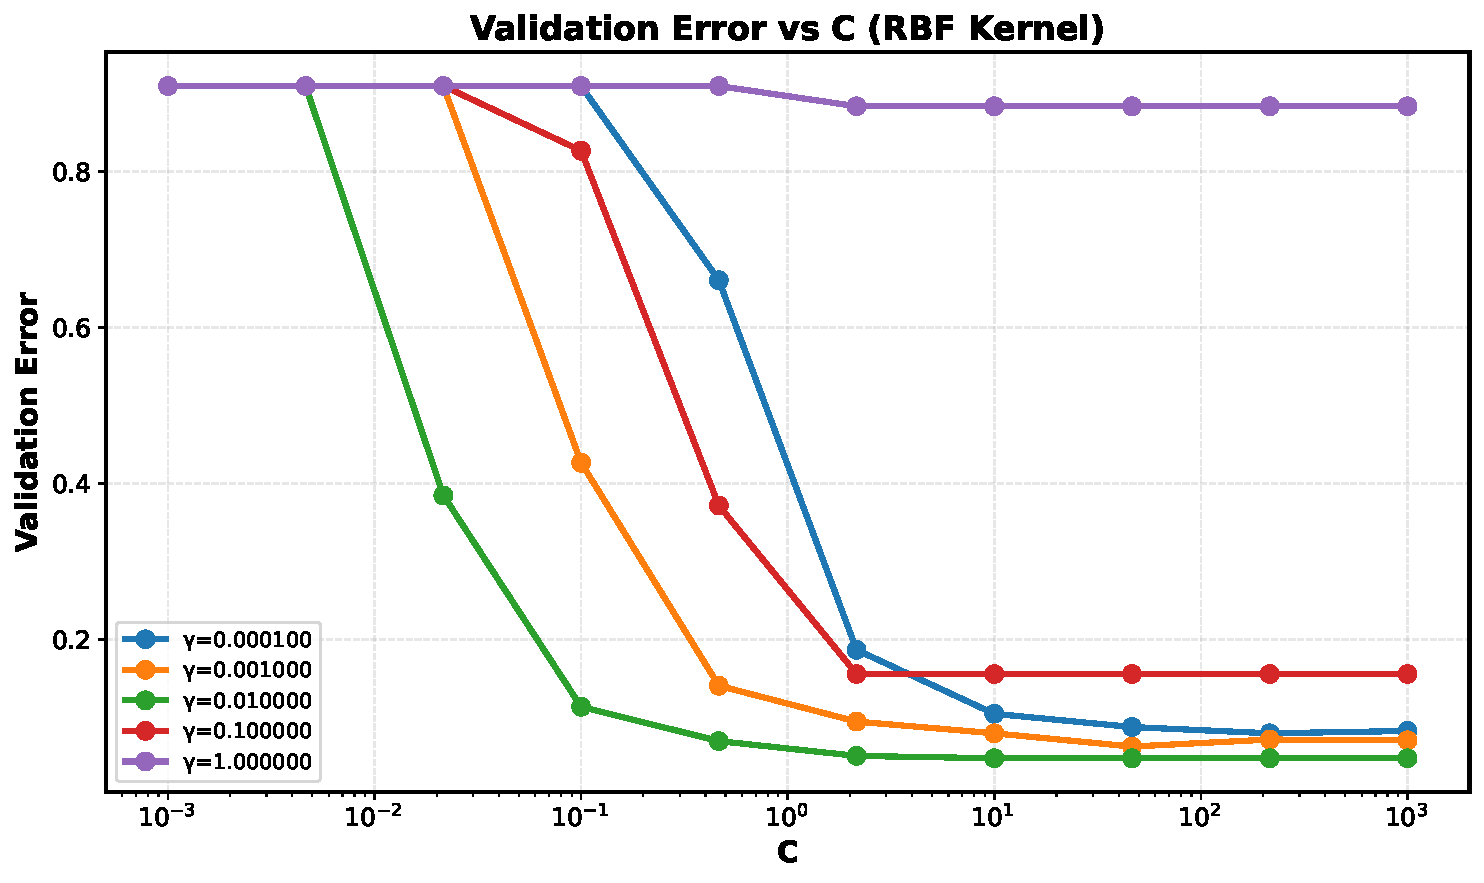
\includegraphics[width=0.85\linewidth]{code release/p3/rbf_validation_error.pdf}
  \caption{Validation error vs. \(C\) across \(\gamma\) values (RBF).}
\end{figure}

\begin{figure}[h]
  \centering
  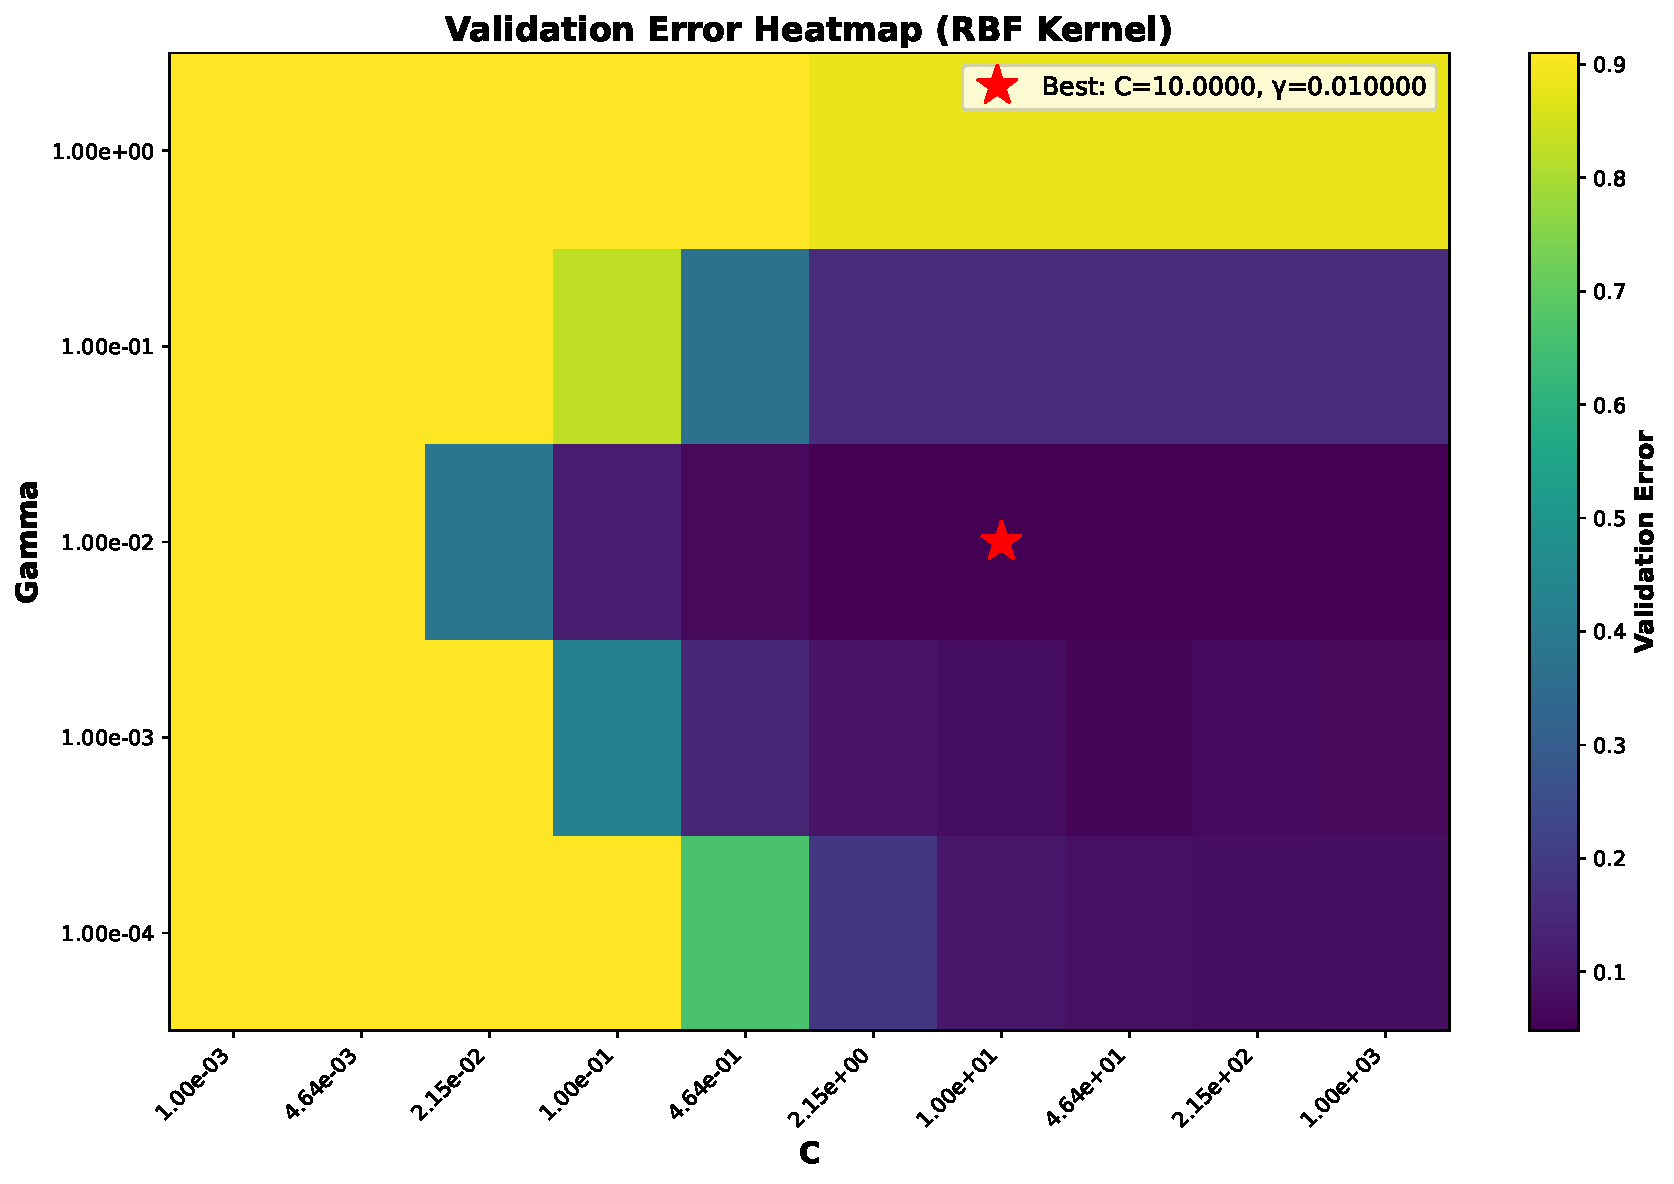
\includegraphics[width=0.9\linewidth]{code release/p3/rbf_heatmap.pdf}
  \caption{Validation error heatmap over \(C\) and \(\gamma\); star marks the best.}
\end{figure}

Key results from the output:
\begin{itemize}
  \item Best: \(C=10.0000\), \(\gamma=0.010000\), Best Val Error: \textbf{0.0480}
  \item Test Error: \textbf{0.0677}, Test Accuracy: \textbf{0.9323}
\end{itemize}

\section*{Conclusion}
Across tasks: (1) Ridge regularization substantially reduces overfitting relative to unregularized high-degree polynomial regression; (2) PCA eigenfaces and SNR curves show improved reconstruction with increasing components and quantify the variance retained; (3) On MNIST, polynomial degree 2 and RBF kernels achieve strong validation and test performance, with RBF slightly better on this split.

\end{document}



